\documentclass{article}
\usepackage[T1]{fontenc}
\usepackage{lmodern}
\usepackage{graphicx}
\usepackage{amsmath,amssymb}
\usepackage[a4paper,margin=2cm]{geometry}
\usepackage[absolute,overlay]{textpos}
\setlength{\TPHorizModule}{1mm}
\setlength{\TPVertModule}{1mm}
\usepackage[indonesian]{babel}
\usepackage{hyperref}
\setlength{\emergencystretch}{2em}
\title{11-Beberapa-block-cipher-bagian3-2026}
\author{pdf\_ppt\_to\_latex}
\date{}

\begin{document}

% --- unit llm 1 ---
% === Halaman 1 (llm) ===

\begin{center}
Bahan kuliah IF4020 Kriptografi

\huge \textcolor{red}{11- Review Beberapa Block Cipher}
\large \textcolor{red}{(Bagian 3: GOST, RC5, RC6, Serpent, dll)}

\vspace{20mm}

\large Oleh: Rinaldi M

\vspace{10mm}

Program Studi Teknik Informatika \\
Sekolah Teknik Elektro dan Informatika \\
Institut Teknologi Bandung \\
2026
\end{center}

\newpage

% --- unit llm 2 ---
% === Halaman 2 (llm) ===

GOST

\newpage

% --- unit llm 3 ---
% === Halaman 3 (llm) ===

\section*{Tinjauan Umum GOST (Magma)}

\begin{itemize}
    \item $GOST = Gosudarstvenny$ $Standard$, artinya standard pemerintah, disebutkan di dalam standard GOST 28147-89 (RFC 5830).
    \item Merupakan algoritma enkripsi $cipher$ blok standard dari negara Uni Soviet dulu (USSR).
    \item Pada mulanya $cipher$ blok ini tidak mempunyai nama, tetapi di dalam standard yang baru, GOST R 34.12-2015 (RFC 7801, RFC 8891), $cipher$ blok ini dinamakan $Magma$.
    \item GOST dikembangkan pada tahun 1970 namun baru dirilis kepada publik pada tahun 1990 setelah Uni Soviet bubar.
    \item Dibuat oleh Soviet sebagai alternatif terhadap algoritma enkripsi standard Amerika Serikat, $DES$.
    \item GOST secara struktural mirip dengan $DES$ (menggunakan jaringan Feistel)
\end{itemize}

\newpage

% --- unit llm 4 ---
% === Halaman 4 (llm) ===

\begin{itemize}
    \item Ukuran blok pesan = 64 bit
    \item Panjang kunci = 256 bit
    \item Jumlah putaran = 32 putaran
    \item Setiap putaran menggunakan kunci putaran.
    \item Kunci putaran sebenarnya hanya ada 8 buah, $K_1$ sampai $K_8$, namun karena ada 32 putaran, maka 8 buah kunci putaran ini dijadwalkan penggunaannya.
\end{itemize}

\vspace{10mm}

\begin{itemize}
    \item Standard GOST yang baru menspesifikasikan \textit{cipher} blok 128-bit yang diberi nama \textit{Kuznyechik}.
\end{itemize}

% deskripsi: Tabel 6.2 Penjadwalan kunci internal GOST yang menunjukkan pemetaan antara nomor putaran (1-32) dengan kunci internal ($K_1$ sampai $K_8$)
% bbox normalisasi: [0.1080, 0.4420, 0.8570, 0.7380]
\begin{textblock*}{157.29mm}(22.68mm,131.27mm)
\noindent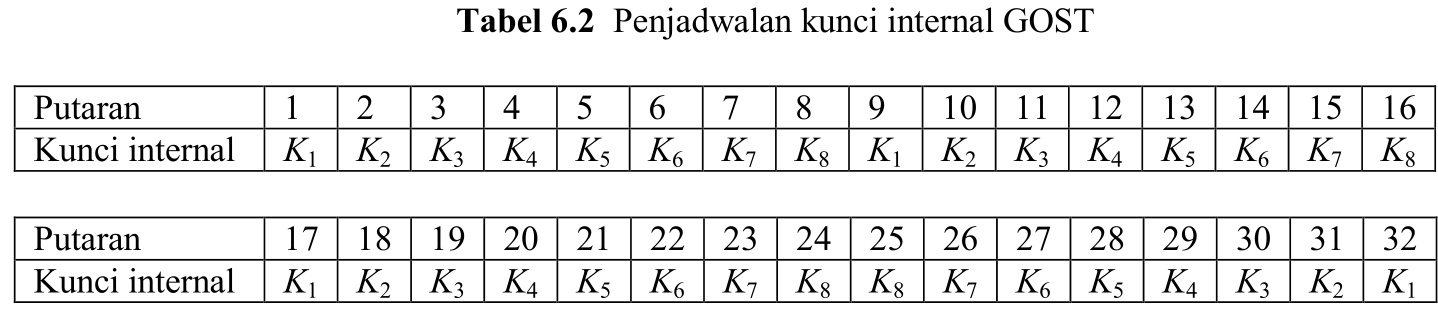
\includegraphics[width=157.29mm,height=87.91mm]{images/llm/page_004_img_01.png}%
\end{textblock*}

\newpage

% --- unit llm 5 ---
% === Halaman 5 (llm) ===

\begin{itemize}
    \item Pembangkitan kunci putaran sangat sederhana.
    \item Kunci eksternal yang panjangnya 256 bit dibagi ke dalam delapan bagian yang masing-masing panjangnya 32 bit.
    \item Delapan bagian ini yang dinamakan $K_1, K_2, \dots, K_8$.
    \item Contoh: $\text{K} = \text{'abcdefghijklmnopqrstuvwxyz123456'}$ \quad $(32 \times 8 \text{ bit} = 256 \text{ bit})$
\end{itemize}

\vspace{5mm}

\begin{minipage}{0.4\textwidth}
    $\text{maka } K1 = \text{'abcd'}$ \\
    $\quad\quad\quad K2 = \text{'efgh'}$ \\
    $\quad\quad\quad K3 = \text{'ijkl'}$ \\
    $\quad\quad\quad K4 = \text{'mnop'}$
\end{minipage}
\begin{minipage}{0.4\textwidth}
    $K5 = \text{'qrst'}$ \\
    $K6 = \text{'uvwx'}$ \\
    $K7 = \text{'yz12'}$ \\
    $K8 = \text{'3456'}$
\end{minipage}

\newpage

% --- unit llm 6 ---
% === Halaman 6 (llm) ===

\vspace{216.81mm}

\begin{itemize}
    \item $\text{GOST menggunakan Jaringan Feistel}$
    \item $\text{Satu putaran GOST:}$
    \[
    \begin{aligned}
    L_i &= R_{i-1} \\
    R_i &= L_{i-1} \oplus f(R_{i-1}, K_i)
    \end{aligned}
    \]
    \vspace{60mm}
    \item $\text{Fungsi } f \text{ terdiri dari}$
    \begin{itemize}
        \item $\text{penjumlahan dalam modulus } 2^{32}$
        \item $\text{substitusi}$
        \item $\text{pergeseran}$
    \end{itemize}
\end{itemize}

\vspace{20mm}
\noindent Keterangan: $\boxed{\begin{smallmatrix} \square \end{smallmatrix}}$ adalah operator penjumlahan dalam modulo $2^{32}$

% deskripsi: Diagram alir struktur Jaringan Feistel untuk satu putaran algoritma GOST, menunjukkan aliran data L dan R, fungsi f dengan substitusi S-Box dan pergeseran sirkuler, serta operasi XOR.
% bbox normalisasi: [0.5500, 0.1400, 0.9400, 0.8700]
\begin{textblock*}{81.90mm}(115.50mm,41.58mm)
\noindent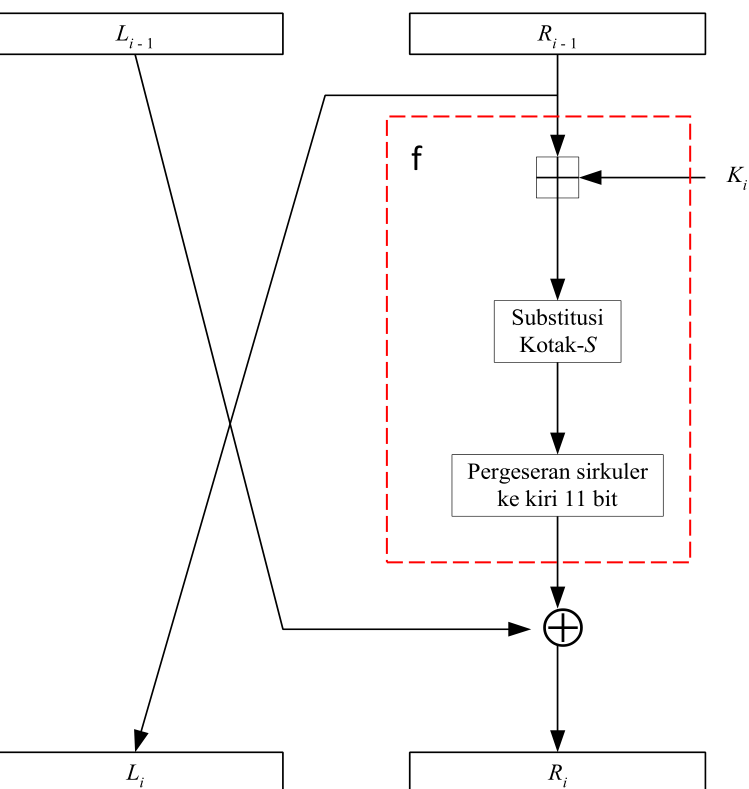
\includegraphics[width=81.90mm,height=216.81mm]{images/llm/page_006_img_01.png}%
\end{textblock*}

\newpage

% --- unit llm 7 ---
% === Halaman 7 (llm) ===

\vspace{196.02mm}

\begin{itemize}
    \item Hasil penjumlahan $R_{i-1}$ dengan $K_i$ menghasilkan luaran yang panjangnya 32 bit.
    \item Luaran ini dibagi menjadi 8 bagian yang masing-masing panjangnya 4 bit.
    \item Setiap 4 bit masuk ke dalam kotak $S$ untuk proses substitusi. Empat bit pertama masuk ke dalam kotak $S$ pertama, 4 bit kedua masuk ke dalam kotak $S$ kedua, demikian seterusnya.
    \item Hasil substitusi setiap kotak $S$ adalah 4 bit. $GOST$ memiliki 8 buah kotak $S$, setiap kotak berisi 16 buah elemen nilai. Setiap kotak berisi permutasi angka 0 sampai 15.
\end{itemize}

\vspace{10mm}

Keterangan: $\square$ adalah operator penjumlahan dalam modulo $2^{32}$

% deskripsi: Diagram blok fungsi enkripsi GOST yang menunjukkan struktur Feistel dengan komponen fungsi f, substitusi kotak-S, pergeseran sirkuler, dan operasi modulo 2^32.
% bbox normalisasi: [0.5400, 0.1600, 0.9900, 0.8200]
\begin{textblock*}{94.50mm}(113.40mm,47.52mm)
\noindent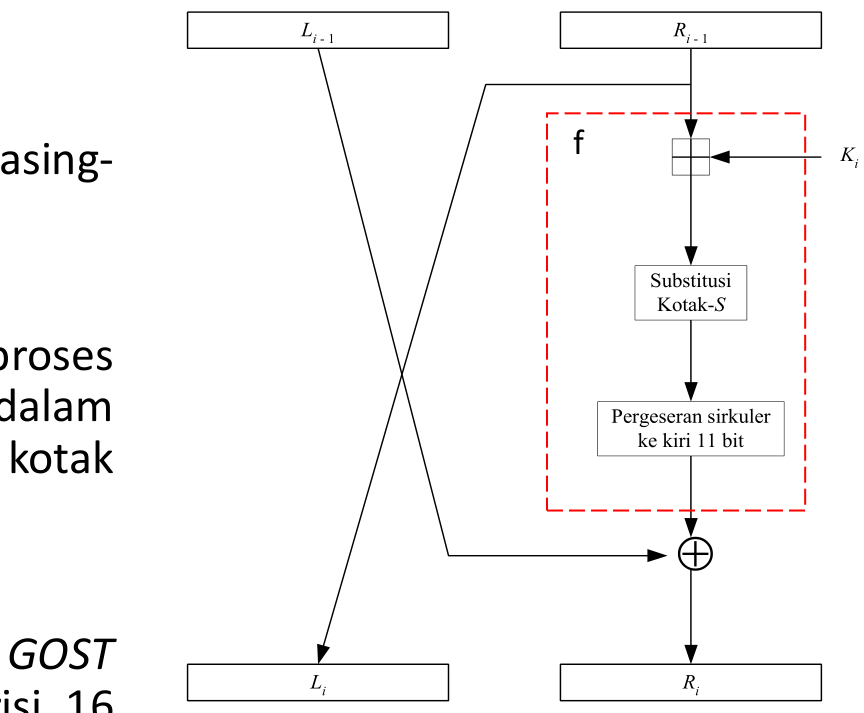
\includegraphics[width=94.50mm,height=196.02mm]{images/llm/page_007_img_01.png}%
\end{textblock*}

\newpage

% --- unit llm 8 ---
% === Halaman 8 (llm) ===

% (tidak ada teks dari model)

% deskripsi: Kumpulan delapan tabel (Kotak-S 1 sampai Kotak-S 8) yang berisi deretan angka acak dalam sel-sel tabel.
% bbox normalisasi: [0.1670, 0.0440, 0.8330, 0.9050]
\begin{textblock*}{139.86mm}(35.07mm,13.07mm)
\noindent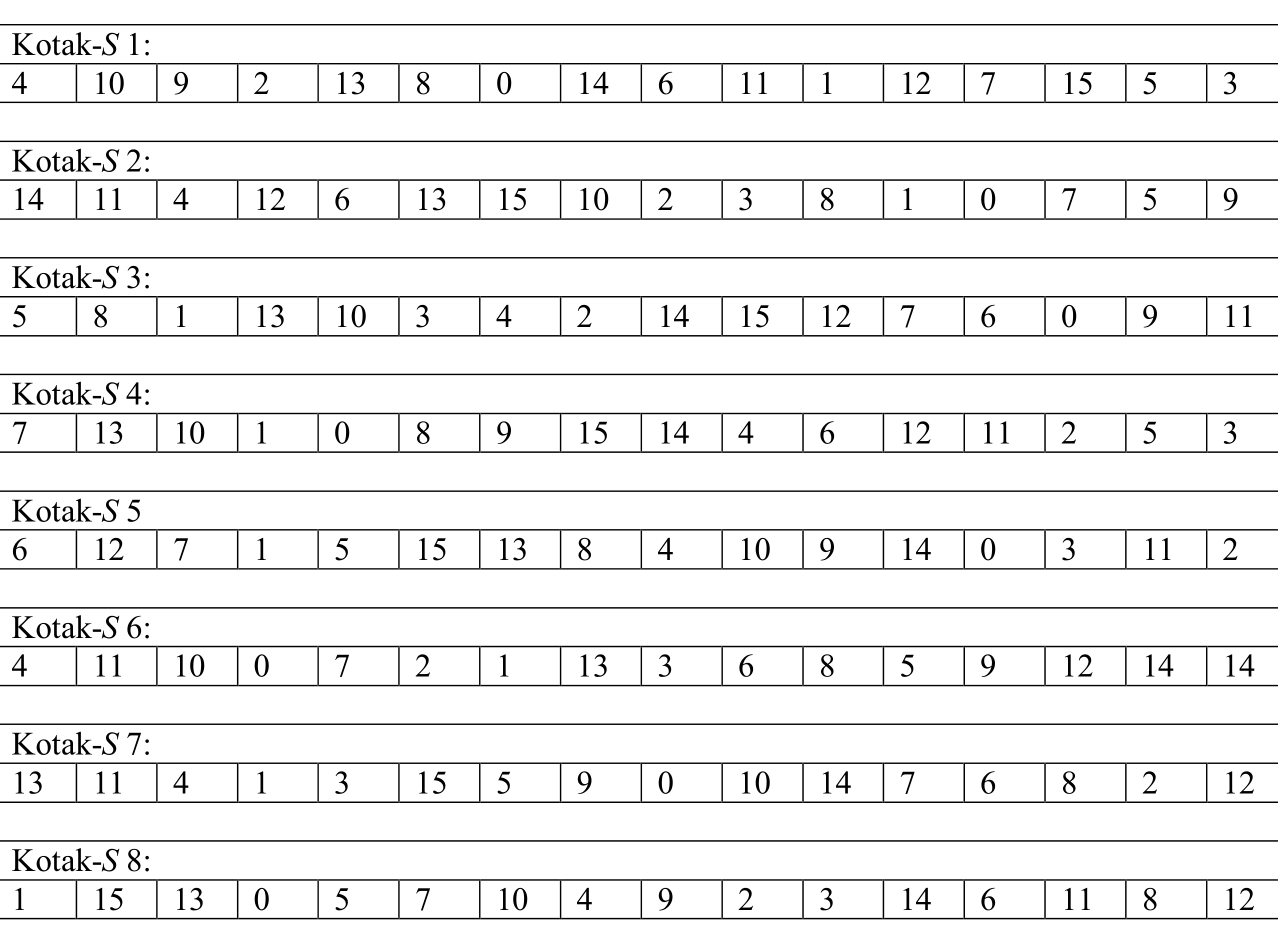
\includegraphics[width=139.86mm,height=255.72mm]{images/llm/page_008_img_01.png}%
\end{textblock*}

\newpage

% --- unit llm 9 ---
% === Halaman 9 (llm) ===

\begin{itemize}
    \item Misalnya pada kotak S pertama, masukannya:
    
    \[ 0010 \quad (\text{nilai desimal 2}) \]
    
    maka luarannya: nilai di dalam elemen ke-2:
    \[ 9 \text{ atau } 1001 \]
\end{itemize}

\vspace{5mm}

\begin{itemize}
    \item Hasil substitusi dari semua kotak S ini digabung menjadi pesan 32-bit.
\end{itemize}

% deskripsi: Tabel Kotak-S 1 yang berisi deretan angka substitusi dari indeks 0 sampai 15.
% bbox normalisasi: [0.0900, 0.5900, 0.9560, 0.6910]
\begin{textblock*}{181.86mm}(18.90mm,175.23mm)
\noindent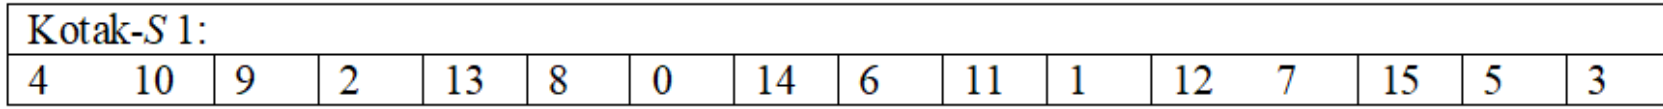
\includegraphics[width=181.86mm,height=30.00mm]{images/llm/page_009_img_01.png}%
\end{textblock*}

\newpage

% --- unit llm 10 ---
% === Halaman 10 (llm) ===

\vspace{204.93mm}

\begin{itemize}
    \item Kemudian pesan 32-bit ini digeser ke kiri sejauh 11 bit secara sirkuler.
    \item Hasilnya kemudian di-XOR-kan dengan $L_{i-1}$ untuk kemudian memberikan bagian cipherteks kanan yang baru, $R_i$. Proses ini diulang sebanyak 32 kali.
    \item Dekripsi merupakan kebalikan dari enkripsi. Dari "bawah" ke "atas" mengikuti jaringan Feistel.
\end{itemize}

\vspace{50mm}

Keterangan: $\boxed{\text{ }\text{ }\text{ }\text{ }}$ adalah operator penjumlahan dalam modulo $2^{32}$

% deskripsi: Diagram alur proses enkripsi jaringan Feistel yang menunjukkan operasi pergeseran sirkuler, substitusi kotak-S, XOR, dan pembaruan nilai L dan R.
% bbox normalisasi: [0.5600, 0.1300, 0.9800, 0.8200]
\begin{textblock*}{88.20mm}(117.60mm,38.61mm)
\noindent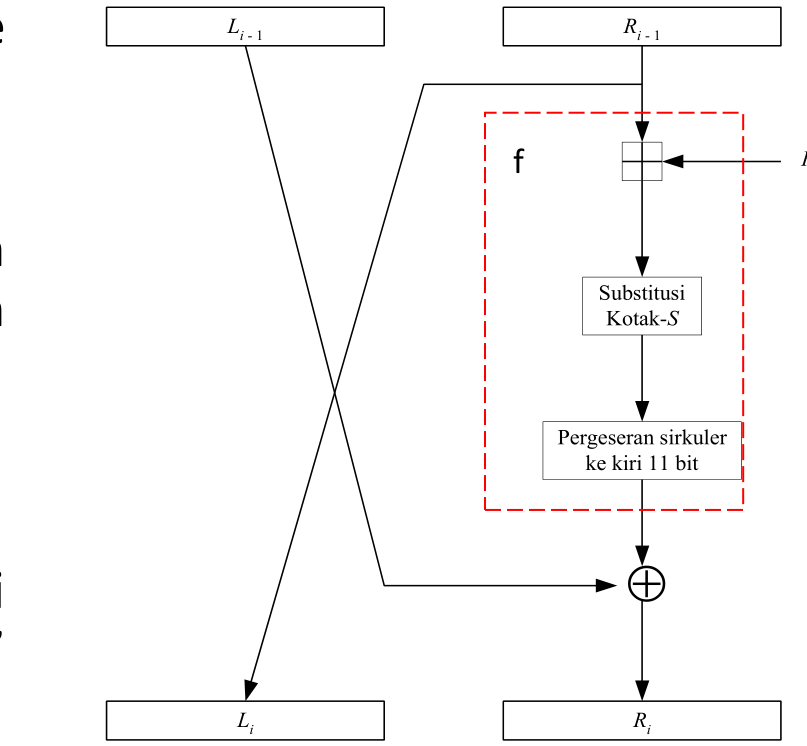
\includegraphics[width=88.20mm,height=204.93mm]{images/llm/page_010_img_01.png}%
\end{textblock*}

\newpage

% --- unit llm 11 ---
% === Halaman 11 (llm) ===

Perbedaan GOST dengan DES:

\begin{enumerate}
    \item Kunci $DES$ 56 bit, sedangkan kunci GOST lebih panjang yaitu 256 bit. Ini menyebabkan \textit{exhaustive key search} terhadap $GOST$ lebih sukar dibandingkan dengan $DES$.
    \item Jumlah putaran DES 16 kali, sedangkan GOST lebih banyak yaitu 32 kali sehingga membuat kriptanalisis menjadi sangat sulit
    \item Kotak S di dalam $DES$ menerima masukan 6 bit dan luaran 4 bit (berukuran $6 \times 4$), sedangkan kotak S di dalam GOST menerima masukan 4 bit dan luaran 4 bit (berukuran $4 \times 4$)
    \item Pembangkitan kunci internal $DES$ rumit, sedangkan di dalam $GOST$ pembangkitan kunci internalnya sederhana
    \item DES mempunyai permutasi yang tidak teratur, sedangkan GOST hanya menggunakan pergeseran 11-bit secara sirkuler
\end{enumerate}

\newpage

% --- unit llm 12 ---
% === Halaman 12 (llm) ===

\section*{Cryptanalysis of GOST}

The latest cryptanalysis of GOST shows that it is secure in a theoretical sense. In practice, the data and memory complexity of the best published attacks has reached the level of practical, while the time complexity of even the best attack is still $2^{192}$ when $2^{64}$ data is available.

Since 2007, several attacks have been developed against reduced-round GOST implementations and/or weak keys.$^{[6][7]}$

In 2011 several authors discovered more significant flaws in GOST, being able to attack the full 32-round GOST with arbitrary keys for the first time. It has even been called ``a deeply flawed cipher'' by Nicolas Courtois.$^{[8]}$ Initial attacks were able to reduce time complexity from $2^{256}$ to $2^{228}$ at the cost of huge memory requirements,$^{[9]}$ and soon they were improved up to $2^{178}$ time complexity (at the cost of $2^{70}$ memory and $2^{64}$ data).$^{[10][11]}$

In December 2012, Courtois, Gawinecki, and Song improved attacks on GOST by computing only $2^{101}$ GOST rounds.$^{[12]}$ Isobe had already published a single key attack on the full GOST cipher,$^{[13]}$ which Dinur, Dunkelman, and Shamir improved upon, reaching $2^{224}$ time complexity for $2^{32}$ data and $2^{36}$ memory, and $2^{192}$ time complexity for $2^{64}$ data.$^{[14]}$

Since the attacks reduce the expected strength from $2^{256}$ (key length) to around $2^{178}$, the cipher can be considered broken. However, for any block cipher with block size of n bits, the maximum amount of plaintext that can be encrypted before rekeying must take place is $2^{n/2}$ blocks, due to the birthday paradox,$^{[15]}$ and none of the aforementioned attacks require less than $2^{32}$ data.

\begin{flushright}
Sumber: Wikipedia
\end{flushright}

\newpage

% --- unit llm 13 ---
% === Halaman 13 (llm) ===

RC5

\newpage

% --- unit llm 14 ---
% === Halaman 14 (llm) ===

\section*{RC5}

\begin{itemize}
    \item $RC5$ dibuat oleh Ronald Rivest dari Laboratorium $RSA$ pada tahun 1994.
    \item Salah satu finalis AES, yaitu RC6, dikembangkan dari RC5
\end{itemize}

\begin{itemize}
    \item Tidak seperti algoritma \textit{cipher} blok lainnya, $RC5$ mempunyai:
    \begin{itemize}
        \item ukuran blok yang variabel (16, 32, 64)
        \item panjang kunci yang variabel (0 sampai 2040 bit)
        \item dan jumlah putaran yang variabel (0 sampai 255).
    \end{itemize}
\end{itemize}

\vspace{5mm}

\begin{tabular}{|l|c|l|}
\hline
\textbf{Parameter} & \textbf{Simbol} & \textbf{Nilai yang dibolehkan} \\ \hline
Ukuran blok (dalam bit) & $w$ & 16, 32, 64 \\ \hline
Jumlah putaran & $r$ & 0, 1, ..., 255 \\ \hline
Panjang kunci eksternal $K$ (dalam $byte$, 1 $byte = 8$ bit) & $b$ & 0, 1, ..., 255 \\ \hline
\end{tabular}

\newpage

% --- unit llm 15 ---
% === Halaman 15 (llm) ===

\section*{Pembentukan Kunci Putaran}

\begin{itemize}
    \item Kunci putaran ada sebanyak $2r + 2$ buah yang masing-masing disimpan di dalam elemen-elemen larik yang dilabeli sebagai $\text{S}[0], \text{S}[1], \dots, \text{S}[t - 1]$ dengan $t = 2r + 2$.
    \item Setiap elemen larik panjangnya satu \textit{word} ($1 \text{ word} = w \text{ bit}$)
\end{itemize}

\vspace{5mm}

% deskripsi: Tabel yang berisi parameter, simbol, dan nilai yang diperbolehkan untuk ukuran blok (w), jumlah putaran (r), dan panjang kunci eksternal K (b).
% bbox normalisasi: [0.1420, 0.6320, 0.7740, 0.8450]
\begin{textblock*}{132.72mm}(29.82mm,187.70mm)
\noindent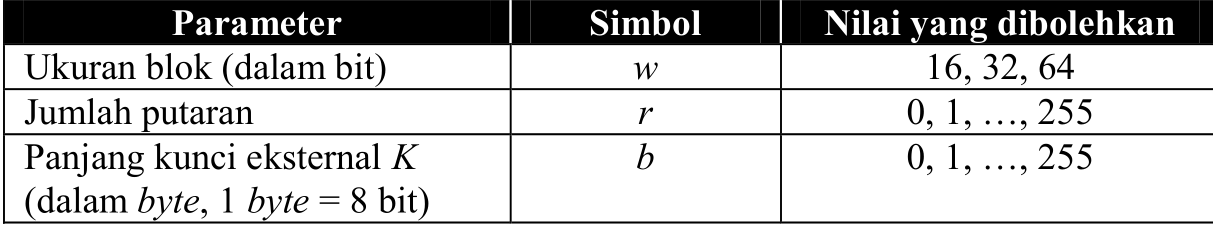
\includegraphics[width=132.72mm,height=63.26mm]{images/llm/page_015_img_01.png}%
\end{textblock*}

\newpage

% --- unit llm 16 ---
% === Halaman 16 (llm) ===

\begin{itemize}
  \item Mula-mula, semua \textit{byte} dari kunci eksternal, $K[0..b-1]$, disalin ke dalam larik $L$ yang berukuran $c$ \textit{word}, $L[0..c-1]$. (ingat: $b$ dalam byte, $c$ dalam word, $c < b$)
  \item lalu \textit{padding} dengan sejumlah 0 jika perlu (\textit{padding} terjadi jika $b$ bukan kelipatan $w$).
  \item Kemudian inisialisasi larik S sebagai berikut:
\end{itemize}

\begin{align*}
S[0] \leftarrow P_w \\
\textbf{for } i \leftarrow 1 \text{ to } t-1 \textbf{ do} \\
\quad S[i] \leftarrow S[i-1] + Q_w \\
\textbf{endfor}
\end{align*}

\vspace{10mm}

% deskripsi: Tabel parameter yang berisi kolom Parameter, Simbol, dan Nilai yang dibolehkan untuk w, r, dan b.
% bbox normalisasi: [0.4010, 0.5700, 0.9810, 0.7920]
\begin{textblock*}{121.80mm}(84.21mm,169.29mm)
\noindent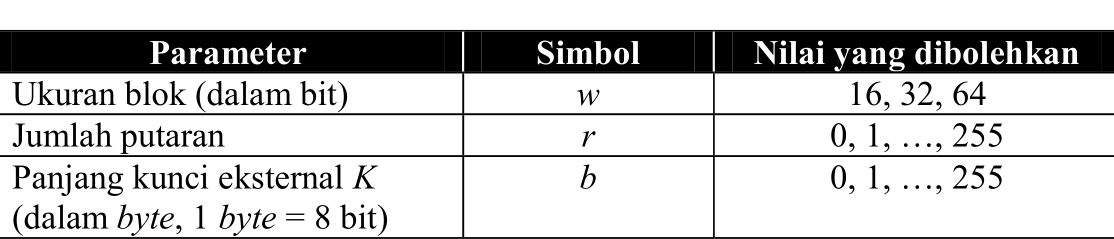
\includegraphics[width=121.80mm,height=65.93mm]{images/llm/page_016_img_01.png}%
\end{textblock*}

\newpage

% --- unit llm 17 ---
% === Halaman 17 (llm) ===

yang dalam hal ini nilai $P_w$ dan $Q_w$ (dalam heksadesimal) berbeda-beda bergantung pada $w$ sebagai berikut [STA98]:

\vspace{10mm}

Konstanta $P_w$ dan $Q_w$ didasarkan pada representasi bilangan alam $e$ dan $\phi$ dalam biner,

\begin{align*}
P_w &= \text{Odd}[(e-2)2^w] \\
Q_w &= \text{Odd}[(\phi-1)2^w]
\end{align*}

\vspace{20.20mm}

yang dalam hal ini,

\[ e = 2.718281828459... \]
\[ \phi = 1.618033988749... = \frac{1+\sqrt{5}}{2} \]

% deskripsi: Tabel nilai Pw dan Qw dalam heksadesimal untuk berbagai nilai w (16, 32, 64).
% bbox normalisasi: [0.1560, 0.2500, 0.8420, 0.4060]
\begin{textblock*}{144.06mm}(32.76mm,74.25mm)
\noindent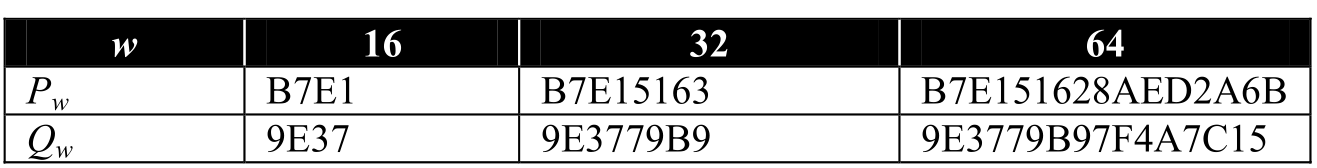
\includegraphics[width=144.06mm,height=46.33mm]{images/llm/page_017_img_01.png}%
\end{textblock*}

% deskripsi: Teks berwarna merah yang menjelaskan definisi fungsi Odd sebagai fungsi yang memberikan integer ganjil terkecil yang dekat dengan input yang diberikan.
% bbox normalisasi: [0.4170, 0.5850, 0.9010, 0.6530]
\begin{textblock*}{101.64mm}(87.57mm,173.74mm)
\noindent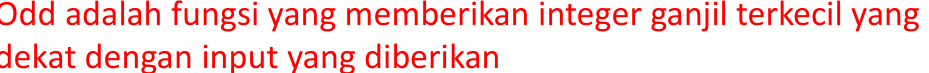
\includegraphics[width=101.64mm,height=20.20mm]{images/llm/page_017_img_02.png}%
\end{textblock*}

\newpage

% --- unit llm 18 ---
% === Halaman 18 (llm) ===

Akhirnya, campurkan $L$ dan $S$ sebagai berikut:

\vspace{160.38mm}

\begin{algorithmic}
\State $i \leftarrow 0$
\State $j \leftarrow 0$
\State $X \leftarrow 0$
\State $Y \leftarrow 0$
\State $n \leftarrow 3 * \max(r, c)$
\For{$k \leftarrow 1$ \textbf{to} $n$ \textbf{do}}
\State $S[i] \leftarrow (S[i] + X + Y) \lll 3$
\State $X \leftarrow S[i]$
\State $i \leftarrow (l + 1) \pmod{t}$
\State $L[j] \leftarrow (L[j] + X + Y) \lll (X + Y)$
\State $Y \leftarrow L[j]$
\State $j \leftarrow (j + 1) \pmod{c}$
\EndFor
\end{algorithmic}

% deskripsi: Potongan kode algoritma pemrosesan array L dan S dengan operasi bitwise rotation dan modulo.
% bbox normalisasi: [0.1700, 0.2600, 0.6100, 0.8000]
\begin{textblock*}{92.40mm}(35.70mm,77.22mm)
\noindent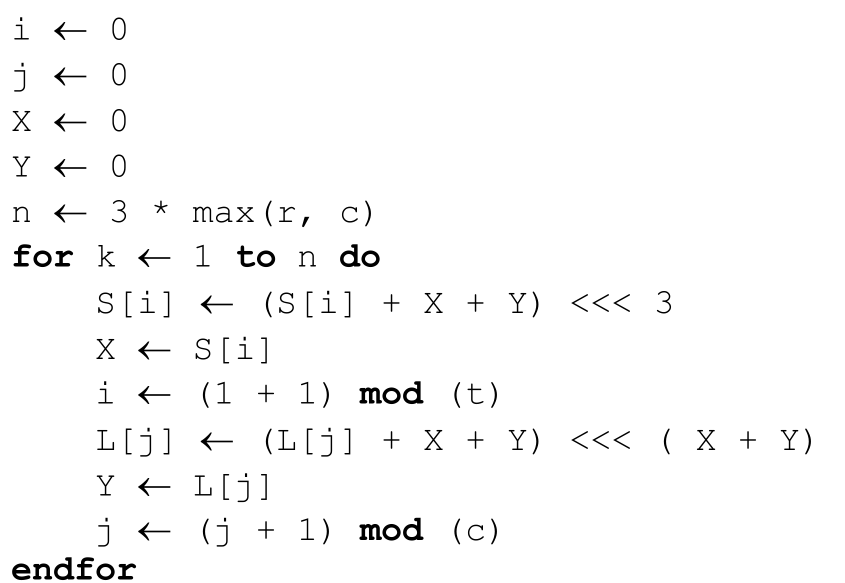
\includegraphics[width=92.40mm,height=160.38mm]{images/llm/page_018_img_01.png}%
\end{textblock*}

\newpage

% --- unit llm 19 ---
% === Halaman 19 (llm) ===

\section*{Enkripsi}

\begin{itemize}
    \item Tinjau $RC5$ dengan ukuran blok 64 bit dan jumlah putaran $r$.
    \item Enkripsi menggunakan kunci putaran $S_0, S_1, \dots, S_{2r+2}$ yang masing-masing panjangnya 32-bit.
    \item Dua kunci putaran digunakan untuk setiap putaran $i = 1, 2, \dots, r$ dan dua buah kunci putaran tambahan sebelum putaran pertama jadi seluruhnya ada $2r + 2$ buah kunci internal.
    \item Untuk melakukan enkripsi, mula-mula blok plainteks dibagi menjadi 2 bagian, $A$ dan $B$, yang masing-masing panjangnya 32 bit. Kemudian masing-masing bagian dijumlahkan (dalam modulo $2^{32}$) dengan $S_0$ dan $S_1$:
    \[
    \begin{aligned}
    A \leftarrow A + S[0] \\
    B \leftarrow B + S[1]
    \end{aligned}
    \]
\end{itemize}

\newpage

% --- unit llm 20 ---
% === Halaman 20 (llm) ===

Selanjutnya untuk setiap putaran 1 sampai $r$ dilakukan operasi $XOR$, pergeseran ke kiri secara sirkuler, dan penjumlahan dalam modulo $2^{32}$ dengan kunci putaran sebagai berikut:

\begin{align*}
\text{for } i \leftarrow 1 \text{ to } r \text{ do}\
\quad A \leftarrow ((A \oplus B) \lll B) + S[2i]\
\quad B \leftarrow ((B \oplus A) \lll A) + S[2i+1]\
\text{endfor}
\end{align*}

\newpage

% --- unit llm 21 ---
% === Halaman 21 (llm) ===

\vspace{273.24mm}

\begin{itemize}
  \item[] \textcolor{red}{\textbf{for} $i \gets 1$ \textbf{to} $r$ \textbf{do}\
  \textcolor{red}{$A \gets ((A \oplus B) \lll B) + S[2i]$}\
  \textcolor{red}{$B \gets ((B \oplus A) \lll A) + S[2i+1]$}\
  \textcolor{red}{\textbf{endfor}}
\end{itemize}

\vspace{20mm}

Cipherteks pada putaran terakhir disimpan di dalam $A$ dan $B$.

Gabungan keduanya adalah blok cipherteks yang berukuran 64 bit.

\vspace{10mm}

Proses enkripsi satu putaran:

% deskripsi: Diagram alur proses enkripsi satu putaran yang menunjukkan operasi XOR, rotasi bit (<<<), dan penjumlahan dengan konstanta S, menghasilkan output A_i dan B_i dari input A_{i-1} dan B_{i-1}.
% bbox normalisasi: [0.5600, 0.0000, 0.8400, 0.9200]
\begin{textblock*}{58.80mm}(117.60mm,0.00mm)
\noindent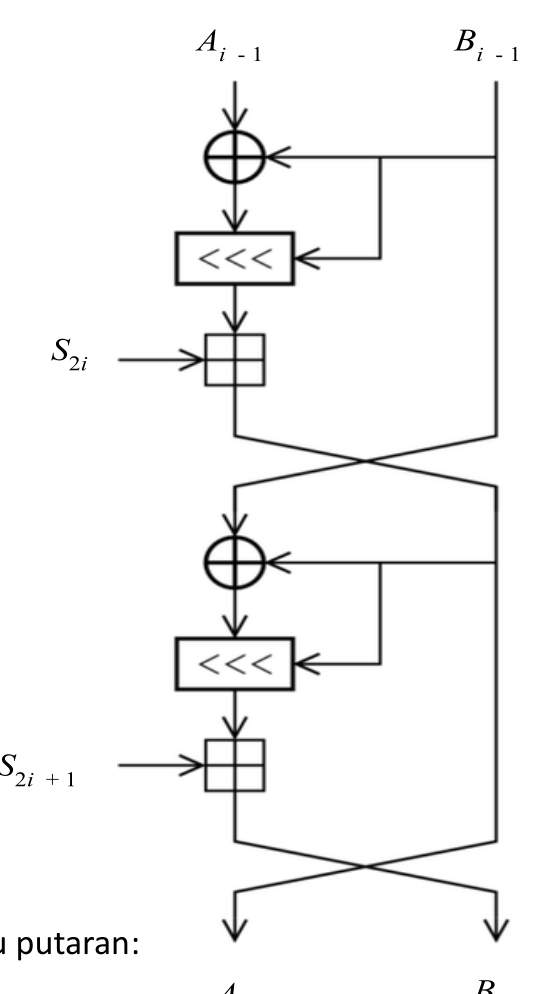
\includegraphics[width=58.80mm,height=273.24mm]{images/llm/page_021_img_01.png}%
\end{textblock*}

\newpage

% --- unit llm 22 ---
% === Halaman 22 (llm) ===

RC6

\newpage

% --- unit llm 23 ---
% === Halaman 23 (llm) ===

\section*{RC6}

\begin{itemize}
    \item RC6 juga dibuat oleh Ronald Rivest, Matt Robshaw, Ray Sidney, dan Yiqun Lisa Yin dari Laboratorium RSA (Rivest, 1998).
    \item RC6 merupakan pengembangan RC5. RC6 dibuat untuk mengikuti kompetisi Advanvced Encryption Standard atau AES (akan dijelaskan pada materi selanjutnya).
    \vspace{10mm}
    \item RC6 melakukan enkripsi terhadap blok data berukuran 128 bit, sedangkan ukuran kuncinya bervariasi 128, 192, 256 sampai 2040 bit. Cara pembangkitan kunci internalnya identik dengan RC5.
    \vspace{10mm}
    \item Secara struktur, RC6 mirip dengan RC5, begitu juga operasi-operasinya seperti XOR, penjumlahan, dan rotasi. RC6 mempunyai operasi tambahan yaitu perkalian.
    \item RC6 dapat dipandang sebagai dua buah RC5 yang dioperasikan secara parallel.
\end{itemize}

\newpage

% --- unit llm 24 ---
% === Halaman 24 (llm) ===

\vspace{100mm}

\textbf{Gambar Jaringan Feistel di dalam RC6.}\\
Fungsi $f$ adalah $f(x) = x(2x + 1)$ (Rivest, 1998)

% deskripsi: Diagram jaringan Feistel yang digunakan dalam algoritma enkripsi RC6, menunjukkan aliran data melalui beberapa ronde dengan operasi XOR, pergeseran bit (rotate), dan fungsi $f$.
% bbox normalisasi: [0.1200, 0.2000, 0.5300, 0.8400]
\begin{textblock*}{86.10mm}(25.20mm,59.40mm)
\noindent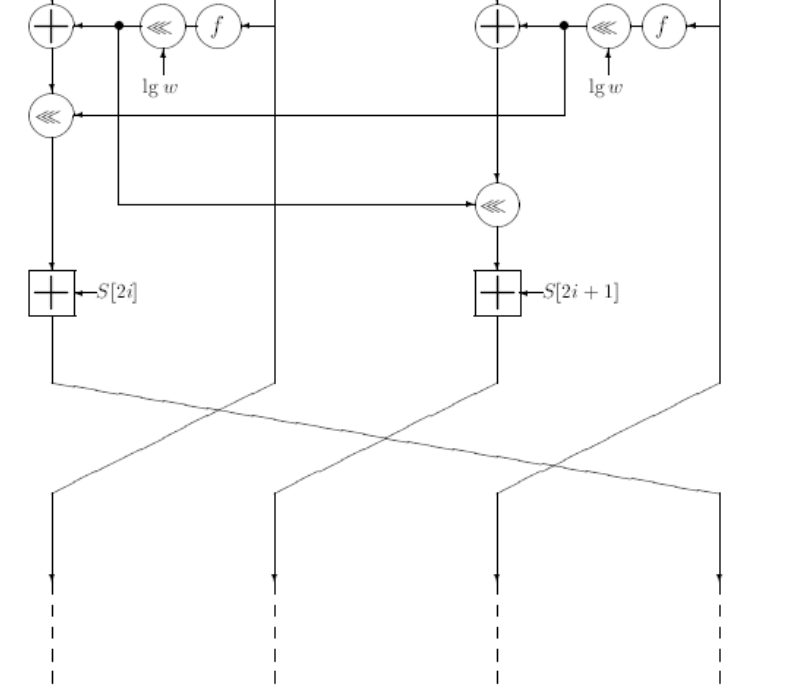
\includegraphics[width=86.10mm,height=190.08mm]{images/llm/page_024_img_01.png}%
\end{textblock*}

\newpage

% --- unit llm 25 ---
% === Halaman 25 (llm) ===

\vspace{168.40mm}

\{ Enkripsi RC6-w/r/b \\
Masukan: Plainteks disimpan di dalam empat register berukuran $w$ bit: $A, B, C$ dan $D$\
\quad $r$ adalah jumlah putaran\\
\quad $S[0, \dots, 2r + 3]$ adalah kunci internal, panjangnya $w$ bit\\
Luaran: Cipherteks disimpan di dalam $A, B, C, D$\
\}

% deskripsi: Algoritma enkripsi RC6 dengan langkah-langkah iterasi for loop dan operasi bitwise.
% bbox normalisasi: [0.1400, 0.3760, 0.6500, 0.9430]
\begin{textblock*}{107.10mm}(29.40mm,111.67mm)
\noindent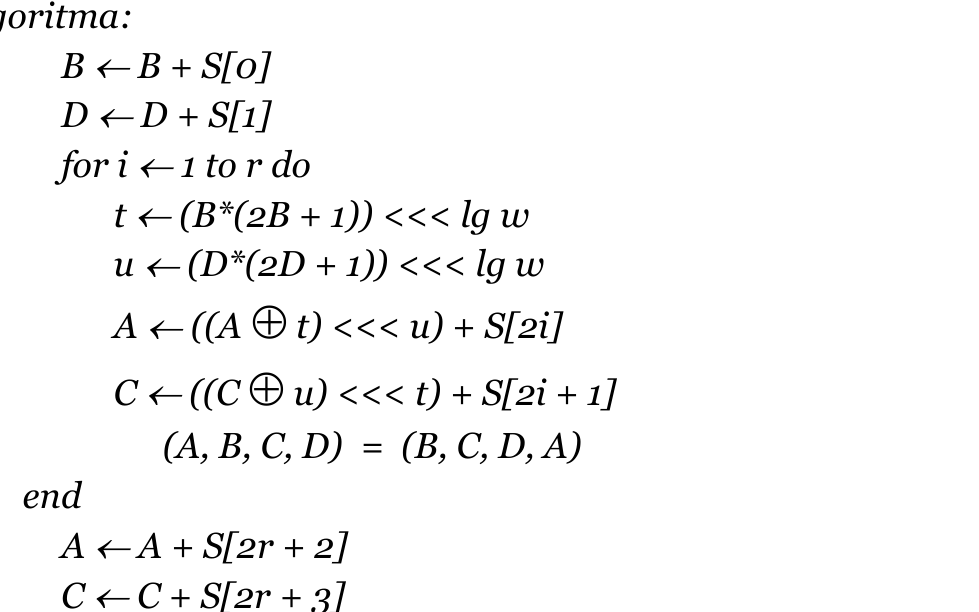
\includegraphics[width=107.10mm,height=168.40mm]{images/llm/page_025_img_01.png}%
\end{textblock*}

\newpage

% --- unit llm 26 ---
% === Halaman 26 (llm) ===

\{ Dekripsi RC6-w/r/b \\
Masukan: Cipherteks disimpan di dalam empat register berukuran $w$ bit: $A, B, C$ dan $D$; $r$ adalah jumlah putaran; $S[0, \dots, 2r+3]$ adalah kunci internal, panjangnya $w$ bit \\
Luaran: Plainteks disimpan di dalam $A, B, C, D$
\}

Algoritma:\
\[ C \leftarrow C - S[2r+3] \\
A \leftarrow A - S[2r+2] \]

\begin{algorithmic}
\For{$i \leftarrow r \text{ downto } 1$}
\State $(A, B, C, D) \leftarrow (D, A, B, C)$
\State $u \leftarrow (D^*(2D + 1)) \lllg lg w$
\State $t \leftarrow (B^*(2B + 1)) \lllg lg w$
\State $C \leftarrow ((C - S[2i + 1]) \gggt t) \oplus u$
\State $\mathbf{A \leftarrow ((A - S[2i]) \gggt u) \oplus t}$
\EndFor
\end{algorithmic}
\[ D \leftarrow D - S[1] \\
B \leftarrow B - S[0] \]

\newpage

% --- unit llm 27 ---
% === Halaman 27 (llm) ===

\textbf{Keterangan:}

\begin{itemize}
    \item $a + b$ adalah penjumlahan dalam modulo $2^w$
    \item $a - b$ adalah pengurangan dalam modulo $2^w$
    \item $a \oplus b$ adalah operasi \textit{bitwise} XOR dari word yang panjangnya $w$ bit
    \item $a \times b$ adalah perkalian dalam modulo $2^w$
\end{itemize}

$a \lll b$ adalah operasi pergeseran $a$ (yang panjangnya $w$ bit) ke kiri secara sirkular sejauh $\log w$ \textit{least significant} bit dari $b$

\vspace{5mm}

$a \ggg b$ adalah operasi pergeseran $a$ (yang panjangnya $w$ bit) ke kanan secara sirkular sejauh $\log w$ \textit{least significant} bit dari $b$

\newpage

% --- unit llm 28 ---
% === Halaman 28 (llm) ===

\begin{center}
\huge Cipher blok lainnya
\end{center}

\newpage

% --- unit llm 29 ---
% === Halaman 29 (llm) ===

\section*{Blowfish}

\begin{itemize}
    \item Dirancang oleh Bruce Schneier tahun 1993.
    \item Ukuran blok plainteks dan cipherteks di dalam Blowfish adalah 64 bit
    \item Panjang kunci 32 sampai 448 bit
    \item Jumlah putaran 16 kali, setiap putaran melakukan operasi substitusi-permutasi
    \item Jumlah kotak S-box adalah 4 buah
\end{itemize}

\newpage

% --- unit llm 30 ---
% === Halaman 30 (llm) ===

P=Plaintext; C=Ciphertext; $K_x \approx$ P-array-entry $x$

\vspace{142.56mm}

$\oplus$ = xor

$\boxplus$ = addition mod $2^{32}$

% deskripsi: Diagram alur algoritma enkripsi blok yang menunjukkan struktur Feistel network dengan satu ronde yang terdiri dari F-Function (S-box 0-3), proses swap, pengulangan 15 ronde tambahan, pembatalan swap terakhir, dan output whitening menggunakan kunci K17 dan K18.
% bbox normalisasi: [0.2100, 0.3600, 0.7500, 0.8400]
\begin{textblock*}{113.40mm}(44.10mm,106.92mm)
\noindent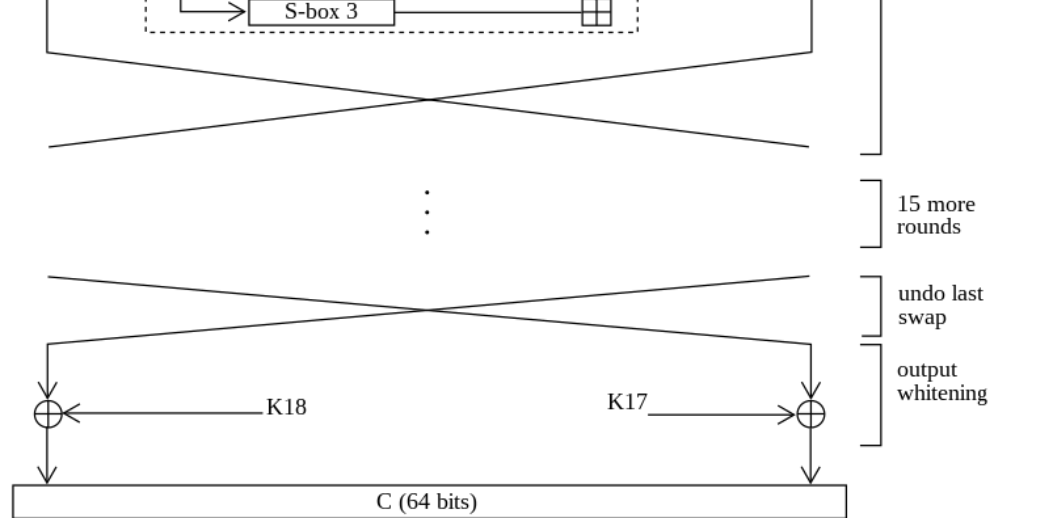
\includegraphics[width=113.40mm,height=142.56mm]{images/llm/page_030_img_01.png}%
\end{textblock*}

\newpage

% --- unit llm 31 ---
% === Halaman 31 (llm) ===

\section*{Serpent}

\begin{itemize}
    \item Salah satu finalis AES (Advanced Encryption Standard)
    \item Dirancang oleh Ross Anderson, Eli Biham, dan Lars Knudsen.
    \item Ukuran blok plainteks dan cipherteks di dalam Serpent adalah 128 bit
    \item Panjang kunci 128, 192, dan 256 bit
    \item Jumlah putaran 32 kali, setiap putaran melakukan operasi substitusi-permutasi
    \item Jumlah kotak S-box adalah 8 buah
\end{itemize}

\newpage

% --- unit llm 32 ---
% === Halaman 32 (llm) ===

\vspace{121.77mm}

Sumber: Introduction to Practical Cryptography, Lecture 3 Block Ciphers

% deskripsi: Diagram alur proses enkripsi block cipher yang menunjukkan tahapan dari Plaintext menjadi Ciphertext, mencakup IP, 32 rounds (whitening, S-Box, Linear Transformation), IP-1, dan keterangan mengenai kunci 256 bit serta operasi bitwise.
% bbox normalisasi: [0.1500, 0.4700, 0.7700, 0.8800]
\begin{textblock*}{130.20mm}(31.50mm,139.59mm)
\noindent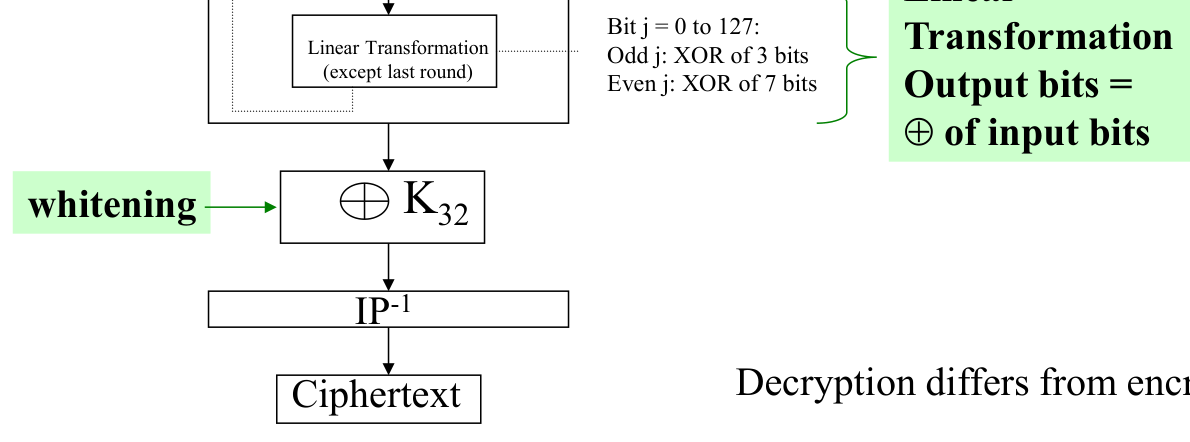
\includegraphics[width=130.20mm,height=121.77mm]{images/llm/page_032_img_01.png}%
\end{textblock*}

\newpage

% --- unit llm 33 ---
% === Halaman 33 (llm) ===

\section*{Twofish}

\begin{itemize}
    \item Salah satu finalis AES (\textit{Advanced Encryption Standard})
    \item Dirancang oleh Bruce Schneier.
    \item Twofish dapat dianggap sebagai kelanjutan dari Blowfish
    \item Ukuran blok plainteks dan cipherteks di dalam Twofish adalah 128 bit
    \item Panjang kunci sampai 256 bit
    \item Jumlah putaran 16 kali, setiap putaran melakukan operasi substitusi-permutasi
    \item Jumlah kotak S-box adalah 5 buah
\end{itemize}

\newpage

% --- unit llm 34 ---
% === Halaman 34 (llm) ===

\vspace{193.05mm}

\begin{itemize}
    \item[\textbf{Legend}] 
    \begin{itemize}
        \item $\bigoplus$ Exclusive-or
        \item $\square$ Addition modulo $2^{32}$
        \item $<<< \text{ Rotation}$
    \end{itemize}
\end{itemize}

% deskripsi: Diagram alur blok kriptografi yang menunjukkan proses enkripsi dari Plaintext (128 bit) menjadi Ciphertext (128 bits), mencakup input whitening, struktur satu ronde dengan S-box, MDS, PHT, rotasi, serta output whitening.
% bbox normalisasi: [0.2100, 0.1400, 0.6300, 0.7900]
\begin{textblock*}{88.20mm}(44.10mm,41.58mm)
\noindent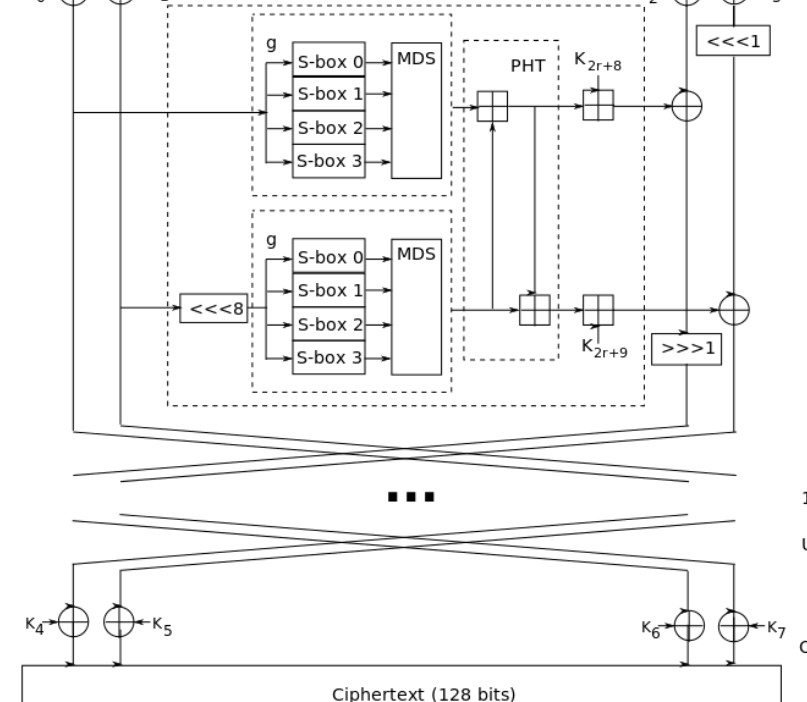
\includegraphics[width=88.20mm,height=193.05mm]{images/llm/page_034_img_01.png}%
\end{textblock*}

\newpage

% --- unit llm 35 ---
% === Halaman 35 (llm) ===

\section*{MARS}

\begin{itemize}
    \item Salah satu finalis AES (\textit{Advanced Encryption Standard})
    \item Dirancang oleh IBM.
    \item Ukuran blok plainteks dan cipherteks di dalam MARS adalah 128 bit
    \item Panjang kunci dari 128 sampai 448 bit (pertambahan 32 bit)
    \item Jumlah putaran 32 kali, setiap putaran melakukan operasi substitusi-permutasi
\end{itemize}

\newpage

% --- unit llm 36 ---
% === Halaman 36 (llm) ===

\vspace{234.63mm}

\section*{Forward Mixing and Backward Mixing}\vspace{10mm}

% deskripsi: Diagram skema proses Forward Mixing dan Backward Mixing pada algoritma kriptografi, menunjukkan aliran data melalui S-boxes, rotasi, penambahan kunci (K), dan operasi XOR.
% bbox normalisasi: [0.0700, 0.1000, 0.8500, 0.8900]
\begin{textblock*}{163.80mm}(14.70mm,29.70mm)
\noindent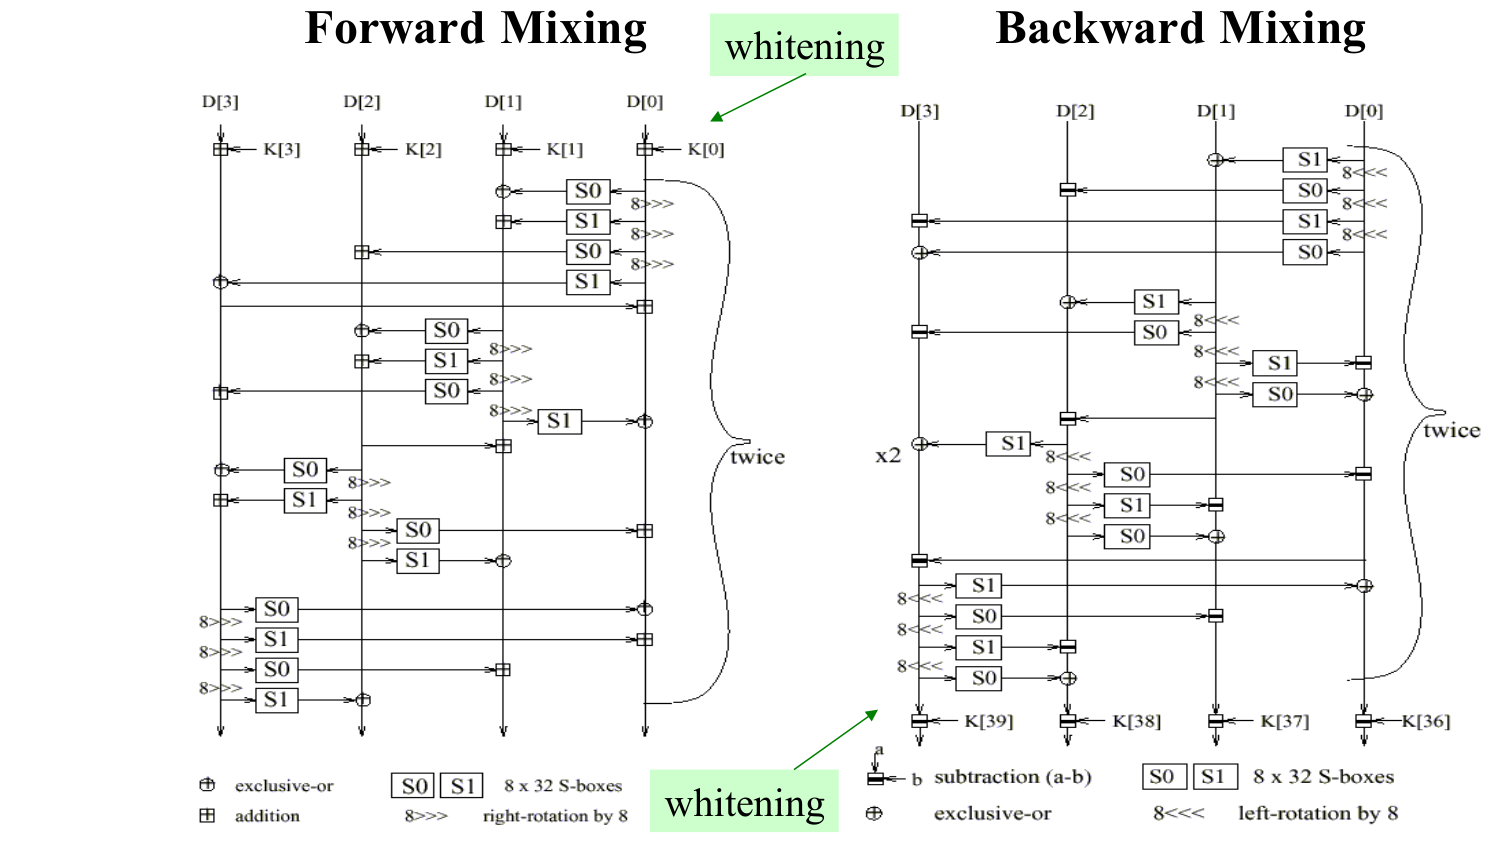
\includegraphics[width=163.80mm,height=234.63mm]{images/llm/page_036_img_01.png}%
\end{textblock*}

\newpage

% --- unit llm 37 ---
% === Halaman 37 (llm) ===

\vspace{141.37mm}

Beberapa algoritma kriptografi simetri:
\vspace{5mm}

% deskripsi: Tabel perbandingan beberapa algoritma kriptografi simetri yang mencakup kolom Cipher, Pembuat, Panjang Kunci, dan Keterangan.
% bbox normalisasi: [0.0700, 0.2380, 0.8890, 0.7140]
\begin{textblock*}{171.99mm}(14.70mm,70.69mm)
\noindent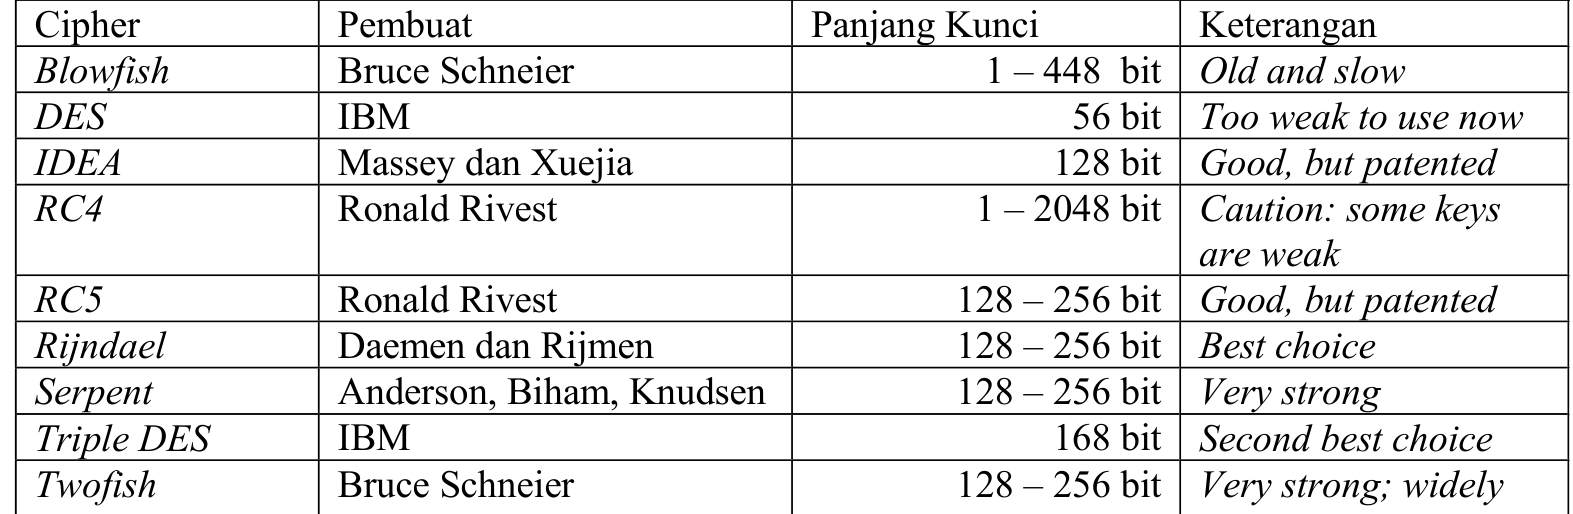
\includegraphics[width=171.99mm,height=141.37mm]{images/llm/page_037_img_01.png}%
\end{textblock*}

\end{document}
